\documentclass[a4paper]{article}
\usepackage[a4paper,margin=0mm]{geometry}
\usepackage{fontspec}
\usepackage{unicode-math}
\usepackage{tikz}
\usepackage[table]{xcolor}
\usepackage[absolute]{textpos}
\usepackage{enumitem}
\usepackage{array}
\usepackage{multirow}

\setmainfont{Libertinus Serif}
\setsansfont{Libertinus Sans}
\setmathfont{Libertinus Math}
\newfontfamily\trackedsans{Libertinus Sans}[LetterSpace=8.0]

\definecolor{accent}{HTML}{602785}
\definecolor{badge}{HTML}{B8A0C8}
\definecolor{ink}{HTML}{2A2E30}

\setlength{\TPHorizModule}{1mm}
\setlength{\TPVertModule}{1mm}
\setlength{\parindent}{0pt}
\pagestyle{empty}

\newcommand{\LCOL}{16mm}
\newcommand{\RCOL}{111mm}
\newcommand{\COLW}{83mm}

\newcommand{\topicheader}[2]{%
\begin{textblock*}{194mm}(16mm,10mm)
\begin{tikzpicture}
\node[fill=accent,text=white,font=\sffamily\bfseries\fontsize{13}{13}\selectfont,
      minimum width=9mm,minimum height=9mm,inner sep=0pt] at (4.5mm,-4.5mm) {#1};
\node[font=\sffamily\bfseries\fontsize{15}{16}\selectfont,text=ink,anchor=west] at (12mm,-4.5mm) {#2};
\end{tikzpicture}
\end{textblock*}
\begin{textblock*}{194mm}(16mm,22.5mm)

\begin{tikzpicture}
\fill[accent] (0,0) rectangle (194mm,0.5mm);
\end{tikzpicture}
\end{textblock*}
}

\newcommand{\pagefooter}[1]{%
\begin{textblock*}{194mm}(8mm,286.41mm)
  
\begin{tikzpicture}
    \fill[accent] (0,0) rectangle (194mm,0.6mm);
  \end{tikzpicture}
\end{textblock*}
\begin{textblock*}{63.59mm}(8mm,288.27mm)
  {\sffamily\bfseries\color{accent}\fontsize{13}{16}\selectfont SAT 1200+}
\end{textblock*}
\begin{textblock*}{10mm}(188mm,288.27mm)
  \centering{\sffamily\color{accent}\fontsize{14}{16}\selectfont #1}
\end{textblock*}
}

\newcommand{\colrule}[2]{%
\begin{textblock*}{1mm}(105mm,#1mm)
\begin{tikzpicture}
\draw[black!65,line width=0.5pt] (0,0) -- (0,#2mm);
\end{tikzpicture}
\end{textblock*}
}

\newcommand{\setkicker}[2]{%
{\sffamily\bfseries\fontsize{12}{14}\selectfont #1.}\ {\itshape\fontsize{11}{14}\selectfont\color{black!75} #2}\par\vspace{2mm}%
}

\setlength{\fboxsep}{1.4pt}
\setlength{\fboxrule}{0.5pt}
\newcommand{\pnum}[1]{\fcolorbox{ink}{white}{\sffamily\bfseries\fontsize{8}{8}\selectfont #1}~}

\newcommand{\qrbox}[1]{%
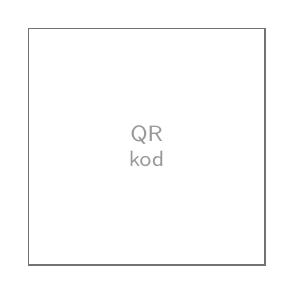
\begin{tikzpicture}
\draw[black!55,line width=0.6pt] (0,0) rectangle (30mm,30mm);
\node[black!40,font=\sffamily\fontsize{8}{9}\selectfont,align=center] at (15mm,15mm) {QR\\kod};
\end{tikzpicture}\\[1.5mm]
{\sffamily\fontsize{9}{11}\selectfont\color{black!70} #1}%
}

\arrayrulecolor{accent}
\setlength{\arrayrulewidth}{0.7pt}
\renewcommand{\arraystretch}{1.35}
\newcommand{\anstitle}[1]{{\sffamily\bfseries\color{accent}\fontsize{11}{13}\selectfont #1}\\[1.3mm]}

\begin{document}

% ================= PAGE 1: Set 1 | Set 2 =================
\topicheader{10}{Ratsional ifodalar va tenglamalar}
\pagefooter{1}
\colrule{32}{238}
\mbox{}%

\begin{textblock*}{\COLW}(\LCOL,32mm)
{\fontsize{12}{15}\selectfont
\setkicker{1-to'plam}{Soddalashtiring -- avval ko'paytuvchilarga ajrating, keyin faqat ko'paytuvchilarni qisqartiring.}

\noindent\pnum{1} $\dfrac{x^2-9}{x+3}=$\\[20mm]
\noindent\pnum{2} $\dfrac{x^2+5x+6}{x+2}=$\\[20mm]
\noindent\pnum{3} $\dfrac{x^2-5x+6}{x^2-4}=$\\[20mm]
\noindent\pnum{4} $\dfrac{2x^2+4x}{x^2-4}=$\\[20mm]
\noindent\pnum{5} $\dfrac{x^2-1}{x^2+2x+1}=$\\[20mm]
\noindent\pnum{6} $\dfrac{x^2-7x+10}{x^2-25}=$
}
\end{textblock*}

\begin{textblock*}{\COLW}(\RCOL,32mm)
{\fontsize{12}{15}\selectfont
\setkicker{2-to'plam}{Ko'paytiring yoki bo'ling.}

\noindent\pnum{1} $\dfrac{x+4}{x-3}\times\dfrac{x-3}{x+1}=$\\[20mm]
\noindent\pnum{2} $\dfrac{x^2-16}{3x}\times\dfrac{x}{x+4}=$\\[20mm]
\noindent\pnum{3} $\dfrac{x-2}{x+5}\times\dfrac{x+5}{x-2}=$\\[20mm]
\noindent\pnum{4} $\dfrac{x^2-9}{x+2}\div\dfrac{x+3}{x+2}=$\\[20mm]
\noindent\pnum{5} $\dfrac{x+1}{x-5}\div\dfrac{x+1}{2x-10}=$\\[20mm]
\noindent\pnum{6} $\dfrac{x^2-4}{5}\div\dfrac{x-2}{10}=$
}
\end{textblock*}

\clearpage

% ================= PAGE 2: Set 3 | Set 4 =================
\topicheader{10}{Ratsional ifodalar va tenglamalar}
\pagefooter{2}
\colrule{32}{238}
\mbox{}%

\begin{textblock*}{\COLW}(\LCOL,32mm)
{\fontsize{12}{15}\selectfont
\setkicker{3-to'plam}{Tenglamani yeching (hali tuzoq yo'q).}

\noindent\pnum{1} $\dfrac{x}{3}+1=\dfrac{x+4}{6}$\\[24mm]
\noindent\pnum{2} $\dfrac{2}{x}+1=3$\\[24mm]
\noindent\pnum{3} $\dfrac{x+1}{x+4}=\dfrac{1}{2}$\\[24mm]
\noindent\pnum{4} $\dfrac{3}{x-1}=\dfrac{2}{x+2}$\\[24mm]
\noindent\pnum{5} $\dfrac{x}{5}+\dfrac{1}{5}=\dfrac{6}{x}$ \textit{(ikkita javob)}
}
\end{textblock*}

\begin{textblock*}{\COLW}(\RCOL,32mm)
{\fontsize{11}{14}\selectfont
\setkicker{4-to'plam}{Yeching va TEKSHIRING -- ba'zi nomzodlar rad etilishi, ba'zilari esa qabul qilinishi kerak. Javobni son yoki ``yechim yo'q'' deb aniq ko'rsating.}

\noindent\pnum{1} $\dfrac{x}{x-3}=\dfrac{3}{x-3}-2$\\[30mm]
\noindent\pnum{2} $\dfrac{x+1}{x-4}=\dfrac{5}{x-4}$\\[30mm]
\noindent\pnum{3} $\dfrac{2x}{x-5}=\dfrac{10}{x-5}+1$\\[30mm]
\noindent\pnum{4} $\dfrac{x+2}{x-1}=3$ \textit{(bu tuzoq emas -- tekshiring)}
}
\end{textblock*}

\clearpage

% ================= PAGE 3: Set 5 | Set 6 (spot the error) =================
\topicheader{10}{Ratsional ifodalar va tenglamalar}
\pagefooter{3}
\colrule{32}{238}
\mbox{}%

\begin{textblock*}{\COLW}(\LCOL,32mm)
{\fontsize{11.5}{14.5}\selectfont
\setkicker{5-to'plam}{Aralash -- har bir band o'z ko'rsatmasiga ega.}

\noindent\pnum{1} Soddalashtiring: $\dfrac{2x^2-8}{x^2-4}=$\\[20mm]
\noindent\pnum{2} Yeching: $\dfrac{4}{x+1}=\dfrac{2}{x-1}$\\[20mm]
\noindent\pnum{3} Ko'paytiring: $\dfrac{x-5}{x+3}\times\dfrac{x+3}{2x}=$\\[20mm]
\noindent\pnum{4} Yeching va tekshiring: $\dfrac{1}{x-2}+\dfrac{1}{x+2}=\dfrac{4}{x^2-4}$\\[20mm]
\noindent\pnum{5} Soddalashtiring: $\dfrac{x^2-6x+9}{x^2-9}=$
}
\end{textblock*}

\begin{textblock*}{\COLW}(\RCOL,32mm)
{\fontsize{11}{14}\selectfont
\setkicker{6-to'plam}{Xatoni toping -- buzilgan qadamni ayting, to'g'ri javobni bering.}

\noindent\pnum{1} $\dfrac{x+5}{x}$ ni soddalashtiring -- ko'rsatilgan yechimda xato bor:\\[1mm]
\hspace*{7mm}\textit{``$x$'larni qisqartiramiz: javob $5$.''}\\[2mm]
\hspace*{7mm}Xato va to'g'ri javob: \makebox[52mm]{\dotfill}\\[6mm]

\noindent\pnum{2} $\dfrac{x^2-4}{x+2}$ ni soddalashtiring -- ko'rsatilgan yechimda xato bor:\\[1mm]
\hspace*{7mm}\textit{``Hammasi qisqaradi, javob $0$.''}\\[2mm]
\hspace*{7mm}Xato va to'g'ri javob: \makebox[52mm]{\dotfill}\\[6mm]

\noindent\pnum{3} $\dfrac{3x}{x-2}=\dfrac{6}{x-2}+x$ ni yeching -- ko'rsatilgan yechimda xato bor:\\[1mm]
\hspace*{7mm}\textit{``Tozalab, $x^2-5x+6=0$, demak $x=2$ yoki $x=3$ -- ikkalasi ham yechim.''}\\[2mm]
\hspace*{7mm}Xato va to'g'ri javob: \makebox[52mm]{\dotfill}\\[6mm]

\noindent\pnum{4} $\dfrac{3x+6}{3x}$ ni soddalashtiring -- ko'rsatilgan yechimda xato bor:\\[1mm]
\hspace*{7mm}\textit{``$3$'larni va $x$'larni qisqartiramiz: javob $6$.''}\\[2mm]
\hspace*{7mm}Xato va to'g'ri javob: \makebox[52mm]{\dotfill}
}
\end{textblock*}

\clearpage

% ================= PAGE 4: Set 6 (item 5 continued) | Set 7 (bonus) =================
\topicheader{10}{Ratsional ifodalar va tenglamalar}
\pagefooter{4}
\colrule{32}{238}
\mbox{}%

\begin{textblock*}{\COLW}(\LCOL,32mm)
{\fontsize{11}{14}\selectfont
\setkicker{6-to'plam (davomi)}{}

\noindent\pnum{5} $\dfrac{x-2}{x+3}\times\dfrac{x+3}{x-2}$ ni ko'paytiring -- ko'rsatilgan yechimda xato bor:\\[1mm]
\hspace*{7mm}\textit{``Hammasi qisqaradi, javob $0$.''}\\[2mm]
\hspace*{7mm}Xato va to'g'ri javob: \makebox[52mm]{\dotfill}
}
\end{textblock*}

\begin{textblock*}{\COLW}(\RCOL,32mm)
{\fontsize{12}{15}\selectfont
\setkicker{7-to'plam}{Bonus / qiyin.}

\noindent\pnum{1} $\dfrac{2}{x-1}-\dfrac{3}{x+1}=1$ \textit{(ikkita javob)}\\[26mm]
\noindent\pnum{2} $\dfrac{x^3-x}{x^2-1}=$\\[26mm]
\noindent\pnum{3} $\dfrac{x+1}{x-3}=\dfrac{x-1}{x+3}$\\[26mm]
\noindent\pnum{4} $\dfrac{1}{x}+\dfrac{1}{x+2}=\dfrac{3}{4}$ \textit{(ikkita javob)}
}
\end{textblock*}

\clearpage

% ================= PAGE 5: Javoblar -- unified answer table + QR =================
\topicheader{10}{Ratsional ifodalar va tenglamalar}
\pagefooter{5}
\mbox{}%

\begin{textblock*}{194mm}(16mm,30mm)
{\bfseries\itshape\color{accent}\fontsize{19}{21}\selectfont\centering Javoblar\par}
\end{textblock*}

\begin{textblock*}{194mm}(16mm,44mm)
{\fontsize{9.5}{12}\selectfont
\centering
\renewcommand{\arraystretch}{1.3}
\begin{tabular}{|>{\centering\arraybackslash}p{24mm}|>{\centering\arraybackslash}p{9mm}|>{\centering\arraybackslash}p{32mm}|>{\centering\arraybackslash}p{9mm}|>{\centering\arraybackslash}p{32mm}|}
\hline
\rowcolor{badge!55}\textbf{To'plam} & \textbf{\#} & \textbf{Javob} & \textbf{\#} & \textbf{Javob}\\
\hline
\multirow{3}{24mm}{\centering 1-to'plam} & 1 & $x-3$ & 2 & $x+3$\\\cline{2-5}
 & 3 & $\frac{x-3}{x+2}$ & 4 & $\frac{2x}{x-2}$\\\cline{2-5}
 & 5 & $\frac{x-1}{x+1}$ & 6 & $\frac{x-2}{x+5}$\\\hline
\multirow{3}{24mm}{\centering 2-to'plam} & 1 & $\frac{x+4}{x+1}$ & 2 & $\frac{x-4}{3}$\\\cline{2-5}
 & 3 & $1$ & 4 & $x-3$\\\cline{2-5}
 & 5 & $2$ & 6 & $2x+4$\\\hline
\multirow{3}{24mm}{\centering 3-to'plam} & 1 & $x=-2$ & 2 & $x=1$\\\cline{2-5}
 & 3 & $x=2$ & 4 & $x=-8$\\\cline{2-5}
 & 5 & \multicolumn{3}{p{48mm}|}{$x=-6$ yoki $x=5$}\\\hline
\multirow{4}{24mm}{\centering 4-to'plam} & \multicolumn{4}{p{74mm}|}{1.\ $x=3$ emas -- mahraj $x-3$ nolga aylanadi. \textbf{Yechim yo'q.}}\\\cline{2-5}
 & \multicolumn{4}{p{74mm}|}{2.\ $x=4$ emas -- mahraj $x-4$ nolga aylanadi. \textbf{Yechim yo'q.}}\\\cline{2-5}
 & \multicolumn{4}{p{74mm}|}{3.\ $x=5$ emas -- mahraj $x-5$ nolga aylanadi. \textbf{Yechim yo'q.}}\\\cline{2-5}
 & \multicolumn{4}{p{74mm}|}{4.\ $x=\frac{5}{2}$ -- mahraj $\frac32\ne0$, \textbf{to'g'ri yechim} (tuzoq emas).}\\\hline
\multirow{3}{24mm}{\centering 5-to'plam} & 1 & $2$ & 2 & $x=3$\\\cline{2-5}
 & 3 & $\frac{x-5}{2x}$ & 4 & \multicolumn{1}{p{32mm}|}{yechim yo'q}\\\cline{2-5}
 & 5 & \multicolumn{3}{p{48mm}|}{$\frac{x-3}{x+3}$}\\\hline
\multirow{5}{24mm}{\centering 6-to'plam} & \multicolumn{4}{p{74mm}|}{1.\ Xato -- $x$ surat $(x+5)$ ning hadi, ko'paytuvchisi emas. To'g'ri: $\frac{x+5}{x}$ allaqachon soddalashtirilgan.}\\\cline{2-5}
 & \multicolumn{4}{p{74mm}|}{2.\ Xato -- $(x+2)$ qisqargach $(x-2)$ qoladi, yo'qolmaydi. To'g'ri: $x-2$.}\\\cline{2-5}
 & \multicolumn{4}{p{74mm}|}{3.\ Xato -- $x=2$ asl mahrajda tekshirilmagan, u nolga aylanadi. To'g'ri: faqat $x=3$.}\\\cline{2-5}
 & \multicolumn{4}{p{74mm}|}{4.\ Xato -- $x$ faqat bitta hadning ko'paytuvchisi. To'g'ri: $\frac{3x+6}{3x}=\frac{x+2}{x}$, ortiq soddalashmaydi.}\\\cline{2-5}
 & \multicolumn{4}{p{74mm}|}{5.\ Xato -- ko'paytuvchilar qisqaradi, lekin natija $1$ bo'ladi, $0$ emas. To'g'ri: $1$.}\\\hline
\multirow{2}{24mm}{\centering 7-to'plam} & 1 & $x{=}{-}3$ yoki $2$ & 2 & $x$\\\cline{2-5}
 & 3 & $x=0$ & 4 & $x{=}{-}\frac43$ yoki $2$\\\hline
\end{tabular}
}
\end{textblock*}

\begin{textblock*}{194mm}(16mm,232mm)
\centering
{\sffamily\fontsize{9.5}{11.5}\selectfont\color{black!70} Video yechimlar va qo'shimcha testlar uchun quyidagi QR kodlarni skanerlang:}\\[4mm]
\begin{minipage}[t]{32mm}\centering\qrbox{YouTube}\end{minipage}%
\hspace{16mm}%
\begin{minipage}[t]{32mm}\centering\qrbox{Telegram}\end{minipage}
\end{textblock*}

\end{document}
